\documentclass{article}
\usepackage[margin=1in]{geometry}
\usepackage{setspace, fancyhdr, hyperref, xcolor, tikz}
\usetikzlibrary{positioning, intersections, calc, arrows}
\usepackage[square,numbers]{natbib}
\bibliographystyle{abbrvnat}
\newcommand{\comment}[1]{}


\newcommand{\thetitle}{Symbolic Manipulation and Computation in the Same Graph}
 
\pagestyle{fancy}
\fancyhf{}
\rhead{\thetitle}
\lhead{Darius Barbano}
\rfoot{Page \thepage}
\doublespacing



\author{Darius Barbano}
\title{\thetitle}
\date{}

\begin{document}

\maketitle
\newpage
\tableofcontents
\newpage

\begin{abstract}
    General artificial intelligence refers to machine intelligence than performs a task as successfully as a human does. A fundamental difference between human neural network and current machine neural networks is that only human networks combine symbolic reasoning with computation. Here we show how a graph can \ldots
\end{abstract}
\newpage


\section{Background}

    \begin{enumerate}
        \item What is symbolic computation?
        
        A symbolic computation is a calculation performed with symbolic representations of values and operations. A simple example would be the expression $(x + 1)(x - 1)$ which would evaluate to $x^2 - 1$, rather than to some numerical result.

        \item What is calculation?
        
        A calculation is a process by which one or more inputs is transformed into one or more results. One may calculate that the product of 5 and 4 is 20.
        
        \item What is meant by a computational class? \textcolor{red}{- do you mean complexity class?}
        
        
    \end{enumerate}
    
     Code for each subsection of this document can be found at \href{https://github.com/DariusBxsci/NeuralNetworkResearch/tree/master/NeuralNets}{NeuralNetworkResearch}. 


\section{Methods}

\subsection{Network Construction}

 Figure \ref{fig:sig-neuron} illustrates a neuron that receives three ordered inputs. 
 
 \begin{figure}[h]
 \centering
 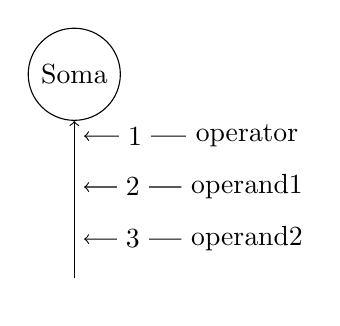
\begin{tikzpicture}

 
    \node[circle, draw=black] (soma) {Soma};
    \node[below= 2cm of soma] (dendrite) {};
    
    \begin{scope}[node distance=1mm and 10mm]
    \node[below right = of soma] (operator) {operator};
    \node[below = of operator] (operand1) {operand1};
    \node[below = of operand1] (operand2) {operand2};
    \end{scope}
    
    
    \draw[->] (dendrite) -> (soma);
    
    
    %nodes along dendrite
    \node (operator'dendrite) at (intersection of operator--soma|-operator and dendrite--soma){};
    
    \node (operand1'dendrite) at (intersection of operand1--soma|-operand1 and dendrite--soma){};
    
    \node (operand2'dendrite) at (intersection of operand2--soma|-operand2 and dendrite--soma){};
    
    
    \draw[->] (operator) -- (operator'dendrite) node[midway, fill=white] {1};
    \draw[->] (operand1) -- (operand1'dendrite) node[midway, fill=white] {2};
    \draw[->] (operand2) -- (operand2'dendrite) node[midway, fill=white] {3};
    
 \end{tikzpicture}
 \caption{Single neuron receiving ordered intputs. \label{fig:sig-neuron}}
\end{figure}

While this model is suitable for biological networks of neurons, a neural network in the computational sense would look more like an abstract syntax tree. In the following diagram, a network of operators and operands form a tree-like structure in which elements at lower levels represent values to manipulate which at higher levels interact with each other through arithmetic operations to produce a result. Any computation which involves a combination of operations on one or more values can be represented in this structure, such as logical operations or large-scale machine learning models.

\newpage

 \begin{figure}
 \centering
 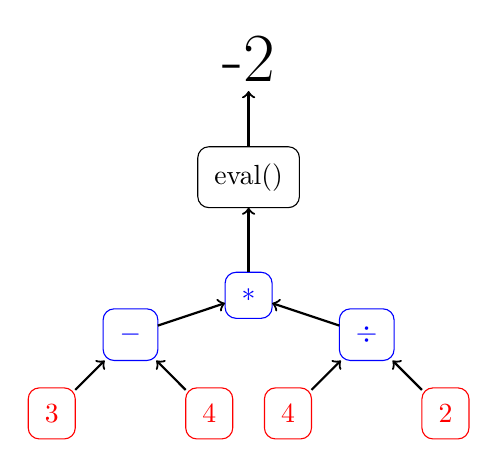
\begin{tikzpicture}

\tikzstyle{bordered} = [shape=rectangle, rounded corners, draw, outer sep=0,inner sep=6,minimum size=15]
\tikzstyle{con} = [thick,->]
\tikzstyle{message} = [shape=rectangle, thick, minimum width=2cm]

	\node [bordered,red] (v1) at (1.5,8) {3};
	\node [bordered,red] (v5) at (3.5,8) {4};
	\node [bordered,red] (v4) at (4.5,8) {4};
	\node [bordered,red] (v3) at (6.5,8) {2};
	
	\node [bordered,blue] (v6) at (5.5,9) {$\div$};
	\node [bordered,blue] (v2) at (2.5,9) {$-$};

	\node [bordered,blue] (v7) at (4,9.5) {$*$};

	\node [bordered,black] (v8) at (4,11) {eval()};

	\node [black] (v9) at (4,12.5) {\Huge -2};

	\draw [con] (v1) edge (v2);
	\draw [con] (v3) edge (v6);
	\draw [con] (v4) edge (v6);
	\draw [con] (v5) edge (v2);

	\draw [con] (v2) edge (v7);
	\draw [con] (v6) edge (v7);

	\draw [con] (v7) edge (v8);

	\draw [con] (v8) edge (v9);

    
 \end{tikzpicture}
 \caption{An Abstract Syntax Tree of arithmetic operations. \label{fig:sig-neuron}} 
\end{figure}

\comment{
 \begin{figure}
 \centering
 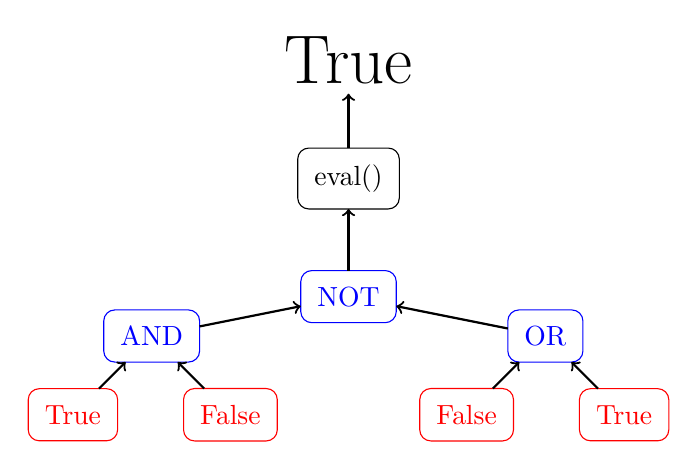
\begin{tikzpicture}

\tikzstyle{bordered} = [shape=rectangle, rounded corners, draw, outer sep=0,inner sep=6,minimum size=15]
\tikzstyle{con} = [thick,->]
\tikzstyle{message} = [shape=rectangle, thick, minimum width=2cm]

	\node [bordered,red] (v1) at (0.5,8) {True};
	\node [bordered,red] (v5) at (2.5,8) {False};
	\node [bordered,red] (v4) at (5.5,8) {False};
	\node [bordered,red] (v3) at (7.5,8) {True};
	
	\node [bordered,blue] (v6) at (6.5,9) {OR};
	\node [bordered,blue] (v2) at (1.5,9) {AND};

	\node [bordered,blue] (v7) at (4,9.5) {NOT};

	\node [bordered,black] (v8) at (4,11) {eval()};

	\node [black] (v9) at (4,12.5) {\Huge True};

	\draw [con] (v1) edge (v2);
	\draw [con] (v3) edge (v6);
	\draw [con] (v4) edge (v6);
	\draw [con] (v5) edge (v2);

	\draw [con] (v2) edge (v7);
	\draw [con] (v6) edge (v7);

	\draw [con] (v7) edge (v8);

	\draw [con] (v8) edge (v9);

    
 \end{tikzpicture}
 \caption{An Abstract Syntax Tree of logical operations. \label{fig:sig-neuron}} 
\end{figure}
}

\textcolor{red}{
Research Idea: In a neural network, rather than just weights being updated through training algorithms, the operations by which the outputs to weights are combined is trained as well. In other words, instead of the inputs to each neuron being added together then put through an activation function, they may be multiplied, subtracted, divided, etc }


\section{Results}

\section{Conclusions}

\bibliography{references}

\end{document}